% =====================================================================
%  latest.tex  --  v0, CONTRIBUTION-FIRST draft
%  "Layered, Evidence-Aware Bluetooth Fingerprinting:
%   Connection-Free Signals, Conflict-Aware Inference, and a
%   Capability Comparison"
%
%  IEEEtran conference format. Standalone, compiles with pdfLaTeX.
%  Framing: the paper foregrounds THIS WORK's contributions (the added
%  signal layers and the evidence chain); the comparison serves to show
%  where those additions differ from prior work. It does NOT claim
%  head-to-head accuracy (different corpora); it compares capability and
%  features, and reports the design contribution.
%
%  STATUS: v0 for advisor feedback. Resolve every \FIXME and VERIFY all
%  references before submission.
% =====================================================================
\documentclass[conference]{IEEEtran}
\IEEEoverridecommandlockouts

\usepackage{cite}
\usepackage{amsmath,amssymb}
\usepackage{array}
\usepackage{booktabs}
\usepackage{graphicx}
\usepackage{url}
\usepackage[T1]{fontenc}
\usepackage{tikz}
\usetikzlibrary{arrows.meta,positioning,fit,backgrounds}
\usepackage{algorithm}
\usepackage{algpseudocode}

\newcommand{\yes}{\checkmark}
\newcommand{\no}{$\times$}
% Third symbol for the signal matrix (Table~\ref{tab:signals}): the source was
% read but does not establish the cell either way. Kept distinct from \no so the
% table never asserts an absence the survey did not actually verify.
\newcommand{\unk}{\textendash}
\newcommand{\FIXME}[1]{\textbf{[FIXME: #1]}}

% Encourage full-width (table*) floats to sit at page tops near their
% reference instead of being deferred to the last (references) page.
\usepackage{stfloats}
\setcounter{topnumber}{2}
\setcounter{dbltopnumber}{2}
\setcounter{totalnumber}{4}
\renewcommand{\topfraction}{0.95}
\renewcommand{\dbltopfraction}{0.95}
\renewcommand{\textfraction}{0.05}
\renewcommand{\floatpagefraction}{0.7}
\renewcommand{\dblfloatpagefraction}{0.7}

\begin{document}

\title{Layered, Evidence-Aware Bluetooth Fingerprinting:\\
Low-Cost Signals and Conflict-Aware Inference}

% TODO before submission: replace the placeholder second author block, or
% delete it if the paper stays single-author. Author ORDER is deliberate and
% is not mine to set - confirm it with your supervisor rather than inheriting
% the order these blocks happen to be written in.
\author{\IEEEauthorblockN{Irem Cesur}
\IEEEauthorblockA{CYSECDIGITAL Research Group\\
Technische Hochschule Mittelhessen (THM)\\
Friedberg, Germany}
\and
\IEEEauthorblockN{[AUTHOR 2 --- NAME]}
\IEEEauthorblockA{[AFFILIATION]\\
{[INSTITUTION]}\\
{[CITY, COUNTRY]}}}

\maketitle

\begin{abstract}
Identifying the operating system of a nearby Bluetooth device supports
security auditing, and existing methods each fall short: they flood the
target, read a single protocol field, or observe the radio, and among the
approaches we surveyed none combines low interaction cost, multi-OS
granularity, and an honest account of uncertainty. We present a layered,
evidence-aware approach extending a baseline active scanner. It adds
version-relevant signals at low marginal cost, an LMP feature bitmap,
chipset/vendor resolution, GATT Appearance and connection parameters, and full
SDP attribute-tree parsing, plus a cached Modalias signal usable only on
re-encounter; and it supplements the fused score with an \emph{evidence chain}
that leaves the prediction unchanged but flags genuine disagreement between
independent signals instead of averaging it away. We then measure when that
mechanism can fire at all, which yields the paper's main finding. Both
originally implemented signal pairs were anchored on GATT~Appearance, present
in 2 of 149 records, so the chain almost never fired despite passing unit
tests; a pair built from two commonly present signals raises coverage to 48\%
of 77 scans, and its first outputs were true positives against our own
derivations. Splitting that coverage by ownership, it fires on 62\% of scans
of our own devices and 10\% of third-party ones. We therefore argue that pair
\emph{co-availability}, not signal quality, bounds this class of inference. A
calibrated \emph{accuracy} evaluation is explicitly not claimed here.
\end{abstract}

\begin{IEEEkeywords}
Bluetooth fingerprinting, BLE privacy, operating-system identification,
evidence-based inference, uncertainty, security audit.
\end{IEEEkeywords}

% =====================================================================
\section{Introduction}
% =====================================================================
Bluetooth, in both its Classic (BR/EDR) and Low Energy (BLE) forms, is
ubiquitous across phones, wearables, peripherals, and IoT devices.
Knowing what a nearby device \emph{is}, its type, vendor, and operating
system, is useful for auditing it: many documented BLE weaknesses are
specific to particular versions or stack implementations, so an OS label
narrows which of them could apply to a given
device~\cite{barua2022blethreats}. We put it no more strongly than that.
An out-of-date OS is neither necessary nor sufficient for a successful
attack, and the survey we cite does not claim otherwise. Bluetooth was
never designed to expose such an identifier, and privacy mechanisms such
as MAC-address randomization and restricted service discovery work
against recovering one~\cite{martin2017macrandom}.

Existing methods each capture part of the picture. Flooding-based
probing reads a device's behavior under stress to recover an OS
version~\cite{kavisankar2024osid}, but at high intrusiveness and with no
representation of uncertainty. Protocol- and GATT-metadata methods
identify a device cheaply~\cite{celosia2019gatt} but stop at a device
model rather than an OS. Radio-frequency
methods~\cite{santanacruz2024jsdivergence} are passive and hard to spoof
but need special hardware and yield a device identity, not an OS.
Runnable tools surface raw data without interpreting it. Across all of them,
two practical properties are missing together: additional
version-relevant signals gathered at low marginal interaction cost, and
an inference step that does something honest when weak signals disagree
rather than averaging them into one verdict.

This paper presents a fingerprinting approach built around those two
properties, extending a baseline active scanner. Our contributions are:

\begin{itemize}
  \item \textbf{Added signal layers at low interaction cost}
  (Section~\ref{sec:layers}): an LMP feature bitmap, chipset/vendor
  resolution, GATT Appearance, GATT preferred connection parameters, and full
  SDP attribute-tree parsing. BR/EDR signals reuse the baseline's connection;
  GATT is a separate LE transport (Table~\ref{tab:transport}). We add
  granularity without a flood, and claim no measured marginal cost.
  \item \textbf{A cache-read signal for re-encounter}
  (Section~\ref{sec:layers}). Modalias is read from the host cache with no
  live connection at scan time, but the cache is populated by a prior
  host-side interaction, so the signal helps on re-encounter and is absent for
  a never-seen target. We do not claim it as a general connection-free
  capability.
  \item \textbf{An evidence chain for conflict-aware inference}
  (Section~\ref{sec:evidence}). Rather than fusing every signal into one
  score, each is labeled supporting, conflicting, primary or unused relative
  to an independent signal; a genuine conflict sets an explicit flag and
  discounts confidence, preserving information a single score destroys.
  \item \textbf{A measurement of when that mechanism can fire at all}
  (Section~\ref{sec:eval}), which yields the paper's main finding: pair
  co-availability, not signal quality, is what bounds this class of
  inference, and it is six times scarcer on unfamiliar devices than on our
  own.
\end{itemize}

\noindent\textbf{Non-goals.} We do not rank methods by accuracy on a shared
corpus (we know of none; Section~\ref{sec:comparison}), defeat MAC
randomization, or claim exact OS-version recovery from Bluetooth metadata.

% =====================================================================
\section{Background and Existing Approaches}\label{sec:related}
% =====================================================================
\emph{Preliminary search; not yet a completed systematic review.}

\textbf{Flooding-based behavioral probing.} Kavisankar et
al.~\cite{kavisankar2024osid} recover an Android version from behavior under
stress: reverse-L2ping support, responses before connection reset, and RSSI
stability while the device is flooded with up to $\sim$3000 packets. It
reaches version granularity but is close to a denial-of-service probe and
emits one verdict with no uncertainty. We instead read version-relevant
signals without a flood and represent disagreement explicitly.

\textbf{Protocol- and GATT-metadata fingerprinting.} Celosia and
Cunche~\cite{celosia2019gatt} fingerprint BLE devices from the GATT
profile; Pferscher and Aichernig~\cite{pferscher2022automata} learn a
protocol state machine via automata learning; Herfurt and Mulliner's
Blueprinting~\cite{herfurt2004blueprinting} hashes Classic SDP records.
These are low-cost but stop at device identity, not OS. We reuse GATT and SDP
as inputs, combine them with LMP and Modalias, and carry them into an
OS/version decision.

\textbf{Radio-frequency and clock-skew methods.} RF
fingerprinting~\cite{santanacruz2024jsdivergence,rusins2023rffingerprint,helluylafont2020sdr}
and clock-skew fingerprinting~\cite{lanze2012clockskew} identify the radio
rather than the protocol: passive and hard to spoof, but needing RF hardware
and yielding a device identity, not an OS. Even that physical fingerprint is
not immutable; a firmware update alone can hide it~\cite{ucsd2024firmware}.

\textbf{Runnable tools.} InsideBlue~\cite{insideblue} dumps GATT data without
interpretation; GhostBLE~\cite{ghostble} reports a privacy posture;
BlueToolkit~\cite{bluetoolkit} tests known CVEs rather than inferring device
identity. The \texttt{nmap} analogy common to this space is only an analogy:
\texttt{nmap}'s OS detection operates on the IP stack and has no Bluetooth
equivalent.

\textbf{The baseline we extend.} Our starting point is an active
scanner\footnote{A prior, unpublished active Bluetooth scanner developed
within the same research project. We treat it as a given baseline and
report only what the present work adds to it; its own design is not a
contribution claimed here.} that performs one point-in-time scan and maps Class-of-Device, a summarized
SDP service list, GATT UUIDs, vendor OUI and LMP version onto a
device/OS/version guess through a single weighted score. It reads no cached
Modalias signal and represents no uncertainty.
Sections~\ref{sec:layers}--\ref{sec:evidence} describe what we add.

We are aware this creates an evaluation problem and prefer to name it rather
than leave it for a reader to hit. A reviewer cannot inspect the baseline, so
a contribution stated purely as a \emph{delta} against it cannot be checked.
We therefore specify the baseline's inputs and decision procedure in full
above, so the difference is at least verifiable from the text, and we state
each contribution in Section~\ref{sec:novelty} in terms that stand on their
own: what the signal is, how it is obtained, and what it lets the system
report. Where a claim genuinely depends on the comparison, we mark it as
such. The alternative, releasing the baseline alongside this work, would
close the gap properly and is the right long-term fix; it is not ours alone
to decide.

% =====================================================================
\section{Approach}\label{sec:approach}
% =====================================================================
\subsection{Overview}
The system performs a layered scan of a target MAC address. Layer~0 is the
baseline active scan; Layers~1--2 add signals read from the connection it
opens, plus one cache-read signal; Layer~3 adds a short behavioral
observation, which the current pipeline reports but does not feed back into
the prediction. The scorer, a fixed-priority rule cascade numeric only in the
Android branch (Section~\ref{sec:scoring}), produces the prediction. The
evidence chain (Section~\ref{sec:evidence}) is computed separately and only
annotates it, lowering the \emph{reported confidence} on a genuine conflict.
It is never an input to the score, so it cannot change which OS or device type
is predicted. Fig.~\ref{fig:arch} shows this structure.

\begin{figure}[t]
\centering
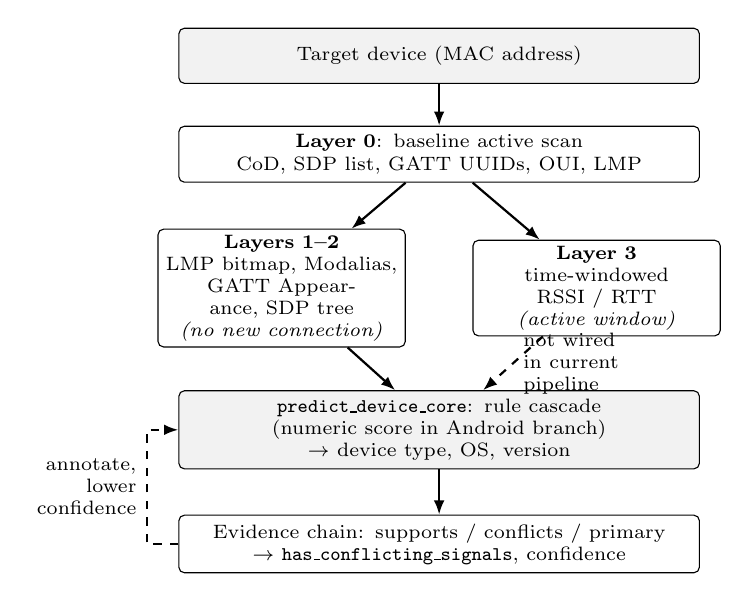
\begin{tikzpicture}[
  font=\scriptsize,
  wide/.style={draw, rounded corners=2pt, align=center, inner sep=3pt,
               text width=6.4cm, minimum height=7mm},
  sig/.style={draw, rounded corners=2pt, align=center, inner sep=2pt,
              text width=3.0cm, minimum height=9mm},
  arr/.style={-{Latex[length=1.8mm]}, thick},
]
\node[wide, fill=black!5] (target) at (0,0) {Target device (MAC address)};
\node[wide] (l0) at (0,-1.25)
  {\textbf{Layer 0}: baseline active scan\\CoD, SDP list, GATT UUIDs, OUI, LMP};
\node[sig] (l12) at (-2.0,-2.95)
  {\textbf{Layers 1--2}\\LMP bitmap, Modalias,\\GATT Appearance, SDP tree\\\emph{(no new connection)}};
\node[sig] (l3) at (2.0,-2.95)
  {\textbf{Layer 3}\\time-windowed\\RSSI / RTT\\\emph{(active window)}};
\node[wide, fill=black!5] (score) at (0,-4.75)
  {\texttt{predict\_device\_core}: rule cascade\\(numeric score in Android branch)\\$\rightarrow$ device type, OS, version};
\node[wide] (chain) at (0,-6.2)
  {Evidence chain: supports / conflicts / primary\\$\rightarrow$ \texttt{has\_conflicting\_signals}, confidence};
\draw[arr] (target) -- (l0);
\draw[arr] (l0) -- (l12);
\draw[arr] (l0) -- (l3);
\draw[arr] (l12) -- (score);
\draw[arr, dashed] (l3) -- node[right, font=\scriptsize, align=left]
  {not wired\\in current\\pipeline} (score);
\draw[arr] (score) -- (chain);
\draw[arr, dashed] (chain.west) -- ++(-0.4,0) |- node[left, pos=0.25,
  align=right, font=\scriptsize] {annotate,\\lower\\confidence} (score.west);
\end{tikzpicture}
\caption{Layered structure. Layers~1--2 reuse the connection Layer~0
opens and feed the scorer (a rule cascade). Layer~3 is a separate active
window; its summary is measured and reported but is \emph{not} carried into
the scorer in the current pipeline (dashed), so no prediction in this paper
rests on it. The evidence chain is computed separately and only annotates the
prediction and lowers reported confidence, never changing which type/OS is
predicted.}
\label{fig:arch}
\end{figure}

\subsection{Added signal layers}\label{sec:layers}
\textbf{Layer 1, hardware and cache-read signals.}
We parse the LMP feature bitmap from the baseline's \texttt{hcitool info}
response: \emph{feature page~0} of the features mask, a BR/EDR field
(\texttt{hcitool info} does not fetch extended pages~1--2, which need Read
Remote Extended Features, and LE-only devices expose LE features instead),
whose named bits include encryption, sniff mode, Secure Simple Pairing and
simultaneous LE/BR-EDR. It comes from a query the baseline already issues, so
it adds parsing cost but no new connection. We also read \emph{Modalias} from
BlueZ's cached \texttt{Device1} properties over D-Bus. This needs no live
connection at scan time but is a cache read: the entry exists only if the
host has previously interacted with the device, and the exact trigger,
pairing, a prior connection or service discovery, we do not establish and do
not claim. It is therefore available on re-encounter, and our measurement
(Section~\ref{sec:eval}) finds it absent for the unfamiliar devices of a cold
sweep, so we do not present it as a general connection-free signal. Where
present we resolve vendor and product against the Bluetooth SIG and USB-IF
assigned-number spaces (kept disjoint), resolve a chipset model where
possible, and run the chronology check of Section~\ref{sec:evidence}.

\textbf{Layer 2, BLE and full SDP signals.}
We read GATT Appearance as a primary device-category signal for BLE-only
devices that expose no Class-of-Device, and GATT preferred connection
parameters as a weak, provisional signal. Where the baseline reads only a
summarized service list, we parse the full SDP attribute tree with a
keyword/version scan over it. These do \emph{not} share one connection: SDP
runs over the BR/EDR connection the baseline already opens, but GATT is an LE
operation on a different transport, read from BlueZ's GATT database, whose
population requires an LE connection. Table~\ref{tab:transport} gives the
access path per signal. We report no measured marginal cost (connections,
queries, wall-clock time); that is future work
(Section~\ref{sec:conclusion}) and until it exists we make no cost claim.

\begin{table}[h]
\centering
\footnotesize
\renewcommand{\arraystretch}{1.15}
\caption{Access path per signal. BR/EDR signals reuse the baseline's
BR/EDR connection; GATT is a separate LE transport; cache reads need no
live connection at scan time.}
\label{tab:transport}
\begin{tabular}{@{}ll@{}}
\toprule
\textbf{Signal} & \textbf{Access path} \\
\midrule
LMP version + feature page 0 & BR/EDR (\texttt{hcitool info}) \\
SDP service list + attribute tree & BR/EDR (\texttt{sdptool}) \\
Class-of-Device & inquiry / D-Bus cache \\
GATT Appearance, conn.\ params, UUIDs & LE (GATT DB, needs LE conn.) \\
Modalias & D-Bus cache (no live conn.) \\
RSSI / RTT (Layer 3) & active (L2CAP / \texttt{hcitool}) \\
\bottomrule
\end{tabular}
\end{table}

\textbf{Layer 3, time-windowed behavioral observation.}
Unlike Layers~1--2 this is a genuinely additional interaction: a short
windowed observation of RSSI and single-packet RTT plus a passive
advertising-interval shift check. It is the least mature layer, and its
confounds (movement, observer effect) we do not claim to have isolated.
It is also, in the pipeline as it stands, not an input to anything: the
summary is streamed to the operator, and the code path that would turn a
high RSSI variance into an evidence-chain conflict is implemented but
unreachable, because the only caller of the scorer passes no behavioral
summary. We report the layer as measurement infrastructure rather than as a
signal layer on the same footing as Layers~1--2, and Table~\ref{tab:signals}
marks RSSI and RTT accordingly.

\subsection{Evidence chain: conflict-aware inference}\label{sec:evidence}
The central methodological element is not a new signal but how signals are
combined. Rather than folding everything into the single score, we generate a
separate \emph{evidence chain} as a post-hoc audit, run in two passes after
the cascade has fixed the prediction.

The first pass is \emph{per signal}: each observed Layer~1--3 signal gets one
record tagging it \emph{primary}, \emph{supports}, \emph{conflicts} or
\emph{unused} relative to the prediction. A signal that was itself a scoring
input for the deciding branch is tagged \emph{primary} and excluded from the
conflict count and confidence penalty, since judging it against a total it
helped produce would be circular. Only signals independent of the prediction
can be tagged \emph{supports} or \emph{conflicts}, and two such checks exist.
The first is chronological: the release year of a Modalias-resolved chipset
against the OS-version bucket derived independently from LMP and profile
flags. It must be one-sided to mean anything, since a chipset older than the
predicted bucket is no conflict (old silicon runs new software) and one newer
than the bucket's \emph{earliest} plausible year holds for almost every
device. Only a chipset released after the \emph{latest} plausible year of the
predicted OS version is a genuine conflict: the device claims, via one signal,
to be older than a component it demonstrably contains. We flag that and note
its false-positive sensitivity when release dates are uncertain. The second
check is textual: a vendor keyword from raw SDP service-name text against the
OUI-resolved vendor.

The second pass is \emph{per pair}: two separately derived device-category
signals are compared with each other rather than with the prediction. Three
pairs are defined and evaluated only when both halves resolve: Class-of-Device
against GATT Appearance, advertised name against GATT Appearance, and
Class-of-Device against advertised name. The first two are independent of the
prediction in the strong sense, since Appearance is consulted only as a
Class-of-Device fallback and so played no part whenever a real Class-of-Device
is present. The third is independent in a weaker but sufficient sense: both
halves fed the prediction, yet neither is computed \emph{from} it, so a
disagreement shows the prediction resting on two contradictory inputs. A
device on which only one category signal resolves yields no pair record,
which is why the chain can be empty even when several signals were read
(Section~\ref{sec:eval}).

A \emph{conflicts} entry from either pass sets an explicit
\texttt{has\_conflicting\_signals} flag and drops the reported confidence one
qualitative level (High / Medium / Low) rather than scaling a numeric
probability, since the weights are not calibrated
(Section~\ref{sec:novelty}). Signals are additionally categorized as
deterministic rules (e.g.\ Class-of-Device major class $\rightarrow$ audio
peripheral) or small provisional adjustments that can nudge a score within a
branch but never flip a prediction. This preserves, and surfaces to an
auditor, the information that two independent weak signals disagreed, which a
single fused score destroys. Algorithm~\ref{alg:chain} states both passes.

\begin{algorithm}[t]
\footnotesize
\caption{Prediction with a separate evidence chain}
\label{alg:chain}
\begin{algorithmic}[1]
\Require observed signal set $S$ (each read once; missing signals absent)
\Require pair set $P$ of separately derived category signals
\State $(\textit{type}, \textit{os}, \textit{ver}, \textit{conf}) \gets
        \Call{PredictDeviceCore}{S}$ \Comment{rule cascade; Android branch scored}
\State $\textit{chain} \gets [\,]$;\quad $\textit{conflict} \gets \textbf{false}$
\Statex \textit{Pass 1: per signal, against the prediction}
\For{each signal $s \in S$ that is relevant to the prediction}
  \If{$s$ was a scoring input for the deciding branch}
     \State append $(s,\textsc{primary})$ to \textit{chain}
            \Comment{excluded from conflict count}
     \State \textbf{continue}
  \EndIf
  \State $\textit{rel} \gets \Call{IndepCheck}{s, \textit{prediction}}$
         \Comment{supports / conflicts / unused}
  \State append $(s,\textit{rel})$ to \textit{chain}
  \State $\textit{conflict} \gets \textit{conflict} \lor
         (\textit{rel} = \textsc{conflicts})$
\EndFor
\Statex \textit{Pass 2: per pair, against each other}
\For{each pair $(a,b) \in P$}
  \If{$a$ or $b$ did not resolve}
     \State \textbf{continue} \Comment{no record; not a conflict}
  \EndIf
  \State $\textit{rel} \gets (a = b)\ ?\ \textsc{supports} : \textsc{conflicts}$
  \State append $((a,b),\textit{rel})$ to \textit{chain}
  \State $\textit{conflict} \gets \textit{conflict} \lor
         (\textit{rel} = \textsc{conflicts})$
\EndFor
\If{\textit{conflict}}
  \State $\textit{conf} \gets \Call{LowerOneLevel}{\textit{conf}}$
         \Comment{High\,$\to$\,Med\,$\to$\,Low}
\EndIf
\State \Return $(\textit{type}, \textit{os}, \textit{ver}, \textit{conf},
        \textit{conflict}, \textit{chain})$
\end{algorithmic}
\end{algorithm}

\subsection{Re-encounter comparison}\label{sec:reencounter}
A device scanned once is scanned again, and the earlier scan is on disk. The
obvious use of it---checking whether the new prediction matches the archived
one---is not available to us, and the reason is the same circularity argument
that shapes the evidence chain. Both predictions come from one scorer, so
their agreement measures self-consistency, not correctness: a scorer with a
systematic bias agrees with itself perfectly. Treating that agreement as
corroboration would be the \emph{primary}-tagging problem of
Section~\ref{sec:evidence} spread across scans rather than within one.

What survives the argument is a comparison of \emph{observations}. We
therefore store, per device, only raw readings---never a prediction, a
confidence, or an advertised name---and compare a new scan against them under
three constraints, each of which is enforced by a unit test rather than
asserted here.

\emph{Only invariant fields are compared.} Modalias, Class-of-Device and the
OUI-resolved vendor are properties of the physical device and cannot
legitimately differ between two scans minutes apart; if they do, at least one
read is wrong whatever the device actually runs, which is a conclusion
available without ground truth. Signals that legitimately vary between scans,
which services answered, whether the LMP read succeeded, RSSI and RTT, are
stored for availability analysis but never compared for equality, since
comparing them would manufacture conflicts out of ordinary variation.

\emph{The result is asymmetric.} A mismatch is recorded as \emph{conflicts}. A
match is recorded as \emph{unused} at weight zero, alongside the undatable
chipset of Section~\ref{sec:evidence}, because a reader agreeing with itself
is not independent corroboration. A device seen for the first time yields no
entry at all: an absent check is not a passed check.

\emph{It can only lower confidence.} Like every other post-hoc check it
annotates and may drop the reported confidence one level; it never enters the
score and never raises confidence, so a prediction does not become better
supported merely because the device has been scanned before.

The store is keyed by a salted HMAC pseudonym rather than by MAC, using the
construction of our release pseudonymizer, so it does not accumulate a second
archive of addresses (Section~\ref{sec:threat}).

\subsection{Scoring model}\label{sec:scoring}
For reproducibility we state the scorer concretely. Device \emph{type} is
decided by a fixed priority order of rule-based branches, first match
wins: (1)~Apple ecosystem (vendor or \texttt{wireless iAP} service);
(2)~Android phone (PBAP/MAP profile, an ``android'' name, or a known
phone vendor when Class-of-Device does not contradict it); (3)~embedded
IoT (chipset vendor); (4)~PC/laptop (host-adapter vendor, an OS name
marker, or an audio source+sink pair); (5)~wearable (CoD major class~7
or ``watch''); (6)~audio (CoD major class~4, an audio profile, or a name
keyword). Branches~1 and 3--6 assign a version by rule (a GATT Device
Information string when present, else an LMP-derived floor); only the
Android branch computes a numeric score, given in Table~\ref{tab:weights}.
Thresholds are compared against the raw integer score $s$ directly,
with no intermediate rescaling, and $s$ is clipped to $[0,105]$ after the
bonuses are added. The complete fixed ladder is: $s\!\ge\!103\Rightarrow$~Android~16; $s\!\ge\!97\Rightarrow$15; $s\!\ge\!87\Rightarrow$14; $s\!\ge\!79\Rightarrow$13; $s\!\ge\!74\Rightarrow$12; $s\!\ge\!70\Rightarrow$11; $s\!\ge\!42\Rightarrow$10; $s\!\ge\!37\Rightarrow$9.0; $s\!\ge\!32\Rightarrow$8.0/8.1;
otherwise 7-or-older. Confidence is the qualitative label High/Medium/Low
(Section~\ref{sec:evidence}).

We report these as the current engineering configuration, \emph{not} as fitted
or validated weights. Three properties of the ladder are enforced by unit
tests rather than asserted in prose, because each corresponds to a defect
present in an earlier revision. (i)~The LMP base is \emph{non-decreasing}: it
previously was not, with LMP~9 scoring 85 against LMP~10's 68, so a device
reporting Bluetooth~5.1 mapped to an \emph{older} Android than one reporting
5.0, a directional error rather than noise. (ii)~Every band is
\emph{reachable}: thresholds were previously compared against a rescaled float
$s'=(s/105)\times10$, placing Android~12 in the raw interval
$[75.075,\,75.6)$, which contains no integer, so the label could never be
emitted. Removing the rescale removes the class of defect, not only this
instance. (iii)~The two provisional adjustments cannot move the estimate by
more than one band; a single point previously moved $75\to76$, i.e.\
Android~11 to Android~13. The structural Device~ID bonus ($+6$) is
deliberately large and \emph{is} permitted to cross a band, so (iii)
constrains only the uncalibrated signals, which is the claim being made about
them.

Re-running the archives under the corrected ladder changes the label for one
device, scanned twice, of the 18 archived scans that reach the Android branch.
It advertises as an OPPO~A5~2020 and reports LMP~9; under the non-monotonic
base it scored 90 and was labelled Android~14, a release postdating the
device, and under the corrected base it scores 73 and is labelled Android~11,
that model's actual final supported release. This is a single consistency
check on a single device, not evidence of accuracy; the paper makes no
accuracy claim.

\begin{table}[h]
\centering
\footnotesize
\renewcommand{\arraystretch}{1.15}
\caption{Android-branch score: base points by LMP version (top,
non-decreasing) plus additive profile bonuses (bottom); two provisional
adjustments are marked. Bonuses sum to at most $+23$, so the raw total is
clipped to 105 after they are applied. Thresholds are compared against the
raw integer score, not a rescaled value. Other device-type branches are
rule-based and use no numeric score (Table~\ref{tab:branches}).}
\label{tab:weights}
\resizebox{\columnwidth}{!}{%
\setlength{\tabcolsep}{4pt}
\begin{tabular}{@{}l *{11}{c}@{}}
\toprule
LMP version & 4 & 5 & 6 & 7 & 8 & 9 & 10 & 11 & 12 & 13 & 14+ \\
Base points & 5 & 10 & 15 & 25 & 48 & 68 & 78 & 85 & 88 & 98 & 105 \\
\bottomrule
\end{tabular}}

\vspace{4pt}
\begin{tabular}{@{}l r@{}}
\toprule
\textbf{Profile / adjustment} & \textbf{Points} \\
\midrule
A2DP / HFP / MAP / PBAP (each) & $+2$ \\
OPP & $+1$ \\
Device ID (DID) profile & $+6$ \\
\quad DID \emph{and} LMP $\ge 11$ & $+6$ extra \\
\emph{Provisional:} simultaneous LE/BR-EDR bit & $+1$ \\
\emph{Provisional:} conn.\ interval min $<15$\,ms & $+1$ \\
\bottomrule
\end{tabular}
\end{table}

\begin{table}[t]
\centering
\footnotesize
\setlength{\tabcolsep}{3.5pt}
\renewcommand{\arraystretch}{1.15}
\caption{Rule set for the five non-Android branches, in priority order, first
match wins; only the Android branch (Table~\ref{tab:weights}) is numeric.
``CoD'' is the Class-of-Device major class, with GATT Appearance mapped onto
the same integers where CoD is absent; ``DIS'' is the GATT Device Information
Service.}
\label{tab:branches}
\begin{tabular}{@{}>{\raggedright\arraybackslash}p{1.35cm}
                  >{\raggedright\arraybackslash}p{3.4cm}
                  >{\raggedright\arraybackslash}p{2.6cm}@{}}
\toprule
\textbf{Branch} & \textbf{Fires when} & \textbf{Version assigned} \\
\midrule
1. Apple &
Vendor/OUI contains ``apple'', or \texttt{wireless iAP} present. Sub-split:
audio if CoD${=}4$, an audio name keyword, or A2DP without a phone indicator
(CoD${=}2$, PBAP, MAP); else iPhone if CoD${=}2$ or iPhone/iPod name; Mac if
CoD${=}1$ or a Mac name; iPad on ``ipad''. &
DIS string when present; else an LMP \emph{floor} only
(${\ge}13\Rightarrow$iOS~17+, ${=}12\Rightarrow$16+, ${=}11\Rightarrow$15+,
else 14-or-older), with macOS/iPadOS equivalents. \\
\addlinespace
3. IoT / embedded &
Vendor matches a known silicon/module maker (Espressif, Texas
Instruments, Nordic, Tuya, Xiaomi, Raspberry). &
None. Reported as \texttt{N/A}: no OS version is claimed. \\
\addlinespace
4. PC / laptop &
Host-adapter vendor (Intel, Realtek, MediaTek, Qualcomm, Broadcom, Atheros,
AzureWave, Rivet/Killer, Lenovo, Dell, HP, Asus, Acer, Microsoft), a
windows/pc/desktop/laptop name token, or both audio \emph{source} and
\emph{sink}. &
Linux marker (BlueZ, Ubuntu, Debian, Linux) $\Rightarrow$ BlueZ stack,
version not claimed. Else Windows by LMP floor: ${\ge}12\Rightarrow$11,
$10\!-\!11\Rightarrow$10, $8\!-\!9\Rightarrow$8.1/10, else 7-or-older. \\
\addlinespace
5. Wearable &
CoD${=}7$ (the specification's Wearable class), or a ``watch'' name token. &
DIS firmware string when present; else none, only the LMP version. \\
\addlinespace
6. Audio &
CoD${=}4$, an audio name keyword, an \texttt{Audio Sink} service, or the
A2DP profile. &
DIS firmware string when present; otherwise none. \\
\addlinespace
--- fallthrough &
No branch matched. &
DIS firmware string when present; otherwise Unknown. \\
\bottomrule
\end{tabular}
\end{table}

\subsection{What is new relative to the baseline}\label{sec:novelty}
The additions over the baseline scanner of Section~\ref{sec:related} are the
signal layers of Section~\ref{sec:layers} and the evidence chain of
Section~\ref{sec:evidence}. The baseline folded every signal into one score
and emitted a single verdict with no uncertainty; the additions raise
granularity at near-zero marginal connection cost and make disagreement
between signals a reported output. The scanner does emit a confidence score,
but it is not calibrated, which we state as a current limitation rather than
a result; Section~\ref{sec:retest} measures how far that label drifts between
two scans of one device minutes apart.

\begin{table}[t]
\centering
\scriptsize
\setlength{\tabcolsep}{2.6pt}
\renewcommand{\arraystretch}{1.12}
\caption{Signals read and outputs produced, per method. Columns:
\textbf{KV}~Kavisankar et al.~\cite{kavisankar2024osid};
\textbf{BL}~the baseline we extend (Section~\ref{sec:related});
\textbf{CC}~Celosia \& Cunche~\cite{celosia2019gatt};
\textbf{PA}~Pferscher \& Aichernig~\cite{pferscher2022automata};
\textbf{BP}~Blueprinting~\cite{herfurt2004blueprinting};
\textbf{IB}~InsideBlue / GhostBLE~\cite{insideblue,ghostble};
\textbf{RF}~RF and clock-skew
methods~\cite{santanacruz2024jsdivergence,rusins2023rffingerprint,lanze2012clockskew};
\textbf{BT}~BlueToolkit~\cite{bluetoolkit};
\textbf{TW}~this work.
A row counts as \yes\ only where the signal is an \emph{input to the method's
own output}, not merely observable to it. \unk\ means the source was read and
does not establish the cell either way; it is kept distinct from \no\ so the
table never asserts an absence our survey did not verify
(Section~\ref{sec:related} states that the survey is preliminary).
Rows~15--18 are outputs, not signals. Rows~12 and~13 are \no\ for this work although the scanner measures both: they are reported as separate metadata and are not inputs to the type/OS/version decision (Section~\ref{sec:layers}).}
\label{tab:signals}
\begin{tabular}{@{}>{\raggedright\arraybackslash}p{2.42cm}
                  *{8}{c}
                  @{\hspace{2pt}}c@{}}
\toprule
& \textbf{KV} & \textbf{BL} & \textbf{CC} & \textbf{PA} & \textbf{BP}
& \textbf{IB} & \textbf{RF} & \textbf{BT} & \textbf{TW} \\
\midrule
\multicolumn{10}{@{}l}{\emph{Input signals}} \\
\midrule
1~~Class-of-Device            & \no  & \yes & \no  & \no  & \unk & \no  & \no & \no  & \yes \\
2~~SDP service list           & \yes & \yes & \no  & \no  & \yes & \no  & \no & \unk & \yes \\
3~~SDP attribute tree         & \no  & \no  & \no  & \no  & \unk & \no  & \no & \no  & \yes \\
4~~LMP version                & \no  & \yes & \no  & \unk & \no  & \no  & \no & \no  & \yes \\
5~~LMP feature bitmap         & \no  & \no  & \no  & \unk & \no  & \no  & \no & \no  & \yes \\
6~~Modalias (host cache)      & \no  & \no  & \no  & \no  & \no  & \no  & \no & \no  & \yes \\
7~~GATT UUIDs                 & \no  & \yes & \yes & \no  & \no  & \yes & \no & \unk & \yes \\
8~~GATT Appearance            & \no  & \no  & \unk & \no  & \no  & \unk & \no & \no  & \yes \\
9~~GATT conn.\ parameters     & \no  & \no  & \unk & \no  & \no  & \unk & \no & \no  & \yes \\
10~GATT Device Info.\ string  & \no  & \no  & \unk & \no  & \no  & \unk & \no & \no  & \yes \\
11~Vendor OUI                 & \no  & \yes & \unk & \no  & \unk & \no  & \no & \unk & \yes \\
12~RSSI                       & \yes & \no  & \no  & \no  & \no  & \no  & \no & \no  & \no  \\
13~Echo / RTT timing          & \yes & \no  & \no  & \unk & \no  & \no  & \no & \no  & \no  \\
14~Radio layer / clock skew   & \no  & \no  & \no  & \no  & \no  & \no  & \yes& \no  & \no  \\
\midrule
\multicolumn{10}{@{}l}{\emph{Outputs}} \\
\midrule
15~Device type / model        & \yes & \yes & \yes & \unk & \yes & \no  & \yes& \no  & \yes \\
16~OS family                  & \yes & \yes & \no  & \no  & \no  & \no  & \no & \no  & \yes \\
17~OS version                 & \yes & \yes & \no  & \no  & \no  & \no  & \no & \no  & \yes \\
18~CVE / vulnerability        & \yes & \no  & \no  & \no  & \no  & \no  & \no & \yes & \no  \\
\bottomrule
\end{tabular}
\end{table}

\begin{table*}[!t]
\centering
\footnotesize
\setlength{\tabcolsep}{5pt}
\renewcommand{\arraystretch}{1.3}
\caption{Method properties that do not reduce to a presence/absence mark.
Which signals each method reads and what it emits is in
Table~\ref{tab:signals}; this table carries only the axes a binary cell would
misrepresent. ``Marginal interaction'' is radio activity beyond passive
discovery; our own figure counts operations issued, which is not the same unit
as the packet count reported for the flooding method and is not comparable to
it. ``Ground-truth corpus'' is the labelled set each source reports,
taken from that source; it is \emph{not} accuracy, and the corpora are
disjoint, so no row is comparable to another as a score. \unk\ marks a cell our
preliminary survey (Section~\ref{sec:related}) did not establish. This work is
the last row.}
\label{tab:cap}
\begin{tabular}{@{}>{\raggedright\arraybackslash}p{3.4cm}
>{\raggedright\arraybackslash}p{2.7cm}
>{\raggedright\arraybackslash}p{4.4cm}
>{\raggedright\arraybackslash}p{3.1cm}
>{\raggedright\arraybackslash}p{3.0cm}@{}}
\toprule
\textbf{Method / tool} & \textbf{Task} & \textbf{Marginal interaction beyond discovery} & \textbf{Ground-truth corpus reported} & \textbf{Uncertainty / conflict} \\
\midrule
Kavisankar et al.~\cite{kavisankar2024osid} & Bluetooth OS + version &
\textbf{High}: SDP and L2ping flooding, up to $\sim$3000 packets, inducing
connection reset on the target (reset at 259 packets on Android~14, 1152 on
Android~10) &
23 devices listed; findings reported for 8, one per Android version &
None: one verdict, always emitted \\
\addlinespace
Baseline scanner (Sec.~\ref{sec:related}) & Bluetooth OS + version &
Medium: one connect-and-query pass &
Not published &
None: single fused score \\
\addlinespace
Celosia \& Cunche~\cite{celosia2019gatt} & BLE device model &
Low: GATT read & \unk & Uniqueness score \\
\addlinespace
Pferscher \& Aichernig~\cite{pferscher2022automata} & Protocol state machine &
Medium: active automata learning & \unk & None \\
\addlinespace
Blueprinting~\cite{herfurt2004blueprinting} & Classic device fingerprint &
Low: SDP read & \unk & None \\
\addlinespace
InsideBlue / GhostBLE~\cite{insideblue,ghostble} & GATT dump / privacy posture &
Low: GATT read & \unk & None \\
\addlinespace
RF and clock-skew~\cite{santanacruz2024jsdivergence,rusins2023rffingerprint,lanze2012clockskew}
& Radio identity &
None: fully passive, but requires RF hardware & \unk & Partial confidence \\
\addlinespace
BlueToolkit~\cite{bluetoolkit} & Vulnerability testing &
Medium: exercises known CVE probes & \unk & None \\
\addlinespace
\textbf{This work} & Bluetooth device type + OS + version &
\textbf{No flood.} 27 radio-facing operations against a fully
responsive target, 35 against an unresponsive one (measured by
instrumenting the scanner; operations, \emph{not} packets). The count is
bounded by our own control flow, not by the target &
8 devices / 43 scans, of which 7 scans carry a verified label &
\textbf{Explicit conflict flag}; confidence uncalibrated, and unstable across
repeat scans (Section~\ref{sec:retest}) \\
\bottomrule
\end{tabular}
\end{table*}



% =====================================================================
\section{Comparison}\label{sec:comparison}
% =====================================================================
The methods above are evaluated on different device sets with different
mechanisms, so their reported accuracies are not comparable and we do not
tabulate them as if they were. We compare what each method \emph{reads} and
\emph{emits} (Table~\ref{tab:signals}), and separately the properties that a
presence/absence mark would misrepresent (Table~\ref{tab:cap}).

Read by column, Table~\ref{tab:signals} says something narrower than a
capability table usually claims. Only two other columns emit an OS version at
all: the flooding strategy of Kavisankar et al.\ and the baseline we extend.
The remaining six address different tasks---device model, protocol state
machine, radio identity, vulnerability---and their columns are mostly empty in
the output block for that reason, not because they attempt our task and fail
at it. We state this plainly because the alternative reading, that this work
fills a gap seven other methods left, would be an artifact of putting adjacent
work in the same table.

Against the two that are comparable, the difference is in the signal block
rather than the output block, and that block is where
Section~\ref{sec:approach} makes its additions. Rows~3, 5, 6 and 8--10---the SDP attribute tree,
the LMP feature bitmap, cached Modalias, and the three GATT metadata
signals---carry a \yes\ in the last column and nowhere else, which is what
Section~\ref{sec:layers} adds. Two of those come with the caveats already
stated: Modalias is a cache read available only on re-encounter, and the
Appearance-bearing pairs fired on almost none of our scans
(Section~\ref{sec:eval}). Rows 12 and 13 separate the two approaches in the
other direction. Kavisankar et al.\ turn RSSI and echo timing into the version
decision itself; we measure both and do not, so those rows are \no\ for this
work. Our scanner reports them as metadata, and the Layer~3 plumbing that
would carry them into the evidence chain exists but is not wired to the
prediction in the shipped pipeline---a gap we state here rather than let the
table imply a capability. The cost difference is real and runs the other way:
they obtain those signals under a flood of up to $\sim$3000 packets that resets
the target's connection, where our whole scan is 27--35 radio-facing
operations with no flood (Table~\ref{tab:cap}).

We do not report a head-to-head run against that method, and the reason is the
method itself. Reproducing it requires flooding third-party devices to
connection reset, which is the one thing our own ethics framing
(Section~\ref{sec:threat}) rules out for the population we scanned. A
comparison on our own devices alone would be a corpus of eight, which settles
nothing. Table~\ref{tab:signals} therefore compares mechanism, not accuracy,
and we make no claim to outperform.

Finally, the \unk\ cells are deliberate. Our survey is preliminary
(Section~\ref{sec:related}), and marking an unverified cell \no\ would assert
an absence we did not check---the failure mode that makes capability tables
easy to win and hard to trust. Every \unk\ is a cell a completed survey should
resolve.

% =====================================================================
\section{Preliminary Signal-Availability Measurement}\label{sec:eval}
% =====================================================================
This section measures one thing: how often the added Layer~1--2 signals are
actually \emph{available} on devices encountered in the wild. It is
\emph{not} an identification-accuracy study, which needs a ground-truthed
corpus and is left to future work (Section~\ref{sec:conclusion}).
Availability is the prior question: a signal that is rarely present cannot
help however good the classifier is.

\textbf{Method.} A standalone two-phase audit passively discovers
Bluetooth addresses, then runs only the Layer~1--2 queries against each,
recording per device whether it was \emph{reached} at all and, if so,
which signals it exposed. Reachability is distinguished from signal
richness explicitly: a device that opens a connection but exposes no
tracked signal (``reached but quiet'') is counted as reached, not as a
connection failure, conflating the two would make ``fraction of reached
devices exposing signal $X$'' partly circular. No payload, content, or
name-to-owner mapping is recorded. Two identifiers \emph{are} recorded and
we name them rather than eliding them: the raw MAC, needed to de-duplicate
within a round, and, in the full-scan archives, the device's own advertised
name. Both can be personal data under Art.~4(1) GDPR~\cite{gdpr2016art4};
see Section~\ref{sec:threat} for the pseudonymization and retention regime
applied to the archive before any release. Two availability rounds were run: an $n{=}18$ pilot in a single office, and an
$n{=}52$ sweep across three locations. Separately, 77 full scans of 21 distinct
devices were archived, and those are the corpus the evidence-chain measurement
below replays; 12 of the 21 are third-party devices, whose scope is stated in
Section~\ref{sec:threat}. Counting every record across both kinds of round
gives 149.

\begin{table}[t]
\centering
\footnotesize
\setlength{\tabcolsep}{4pt}
\renewcommand{\arraystretch}{1.2}
\caption{Signal availability in the wild. Percentages are of the round's
$n$. ``Reached but quiet'' devices are reached yet expose no Layer~1--2
signal. Modalias is a host-cache read, not a live signal, and is reported
against \emph{both} denominators: it can be present for an address we never
reached live, so ``of all addresses'' and ``of reached addresses'' answer
different questions and a single figure silently picks one. Counts are given
raw; at these $n$ a percentage would read as an estimate it cannot support.}
\label{tab:avail}
\begin{tabular}{@{}>{\raggedright\arraybackslash}p{4.7cm} r r@{}}
\toprule
& \textbf{Pilot ($n{=}18$)} & \textbf{Sweep ($n{=}52$)} \\
\midrule
Never reached by pipeline & 16 & 46 \\
\quad 95\% CI (of $n$) & [65,99]\% & [77,96]\% \\
Reached & 2 & 6 \\
\quad exposed $\ge$1 Layer-2 signal & 2 & 2 \\
\quad reached but quiet & 0 & 4 \\
\midrule
GATT Appearance present & 1 & 0 \\
SDP service name present & 1 & 2 \\
\midrule
\multicolumn{3}{@{}l}{\emph{Modalias, both denominators}} \\
\quad present, of all addresses & 8/18 & 0/52 \\
\quad present, of reached addresses & 2/2 & 0/6 \\
\bottomrule
\end{tabular}
\end{table}

\textbf{Findings.} Table~\ref{tab:avail} shows that, in this pipeline,
reachability rather than signal richness is the first-order constraint:
16 of 18 (89\%, 95\% CI [65,99]) and 46 of 52 (88\%, 95\% CI [77,96])
addresses were never reached. One caveat is essential to how this is
read: ``never reached'' here means the address was seen in passive
discovery but never entered BlueZ's object tree
(\texttt{UnknownObject}), a failure of \emph{our BlueZ-based pipeline}
to open a channel, which is not the same as a proven device refusal, and
could also reflect non-connectable advertising or a tool limitation.
Until a positive control (a known-connectable device on the same
pipeline) is run, we state the result as ``not reached by this
pipeline,'' not ``refused connection.'' The two \emph{signal-bearing}
addresses in the sweep (of the six reached) were both read over SDP, so
the reached set also mixes transport paths; we do not over-generalize
from it.

The Modalias row is the sharpest and most self-critical result: present
for 8 of 18 pilot addresses (44\%, 95\% CI [22,69]) but 0 of 52 sweep
addresses (95\% CI [0,7]). The pilot ran in the researcher's own office, where those devices
were already paired to the host; the multi-location sweep met unfamiliar
devices and found no cached Modalias at all. This is direct empirical
support for the scope stated in Section~\ref{sec:layers}: Modalias helps
on re-encounter and is absent on first contact, so it is not a general
connection-free signal.

\textbf{Evidence-chain firing.} We replayed the current inference build over
every archive and recorded, per signal, how often each entry fired and, when
it did not, which precondition was missing. That distinction is the point: a
signal silent because its input was never captured is an availability result,
whereas one silent while its inputs were present would be a defect. No signal
was silent while its preconditions held.

The mechanism is not defective. Unit tests confirm it emits a
\emph{supporting} entry for an agreeing independent pair, a
\emph{conflicting} entry for a disagreeing one, no pair entry when only one
side is present, a non-corroborating \emph{primary} entry for the dependent
case, and an empty chain on empty input. An earlier draft attributed the
empty archive to conflicts being rare; that explanation, and the coding-error
diagnosis it implied, were both wrong. Of 77 archived full scans over 21
devices, only~11 were collected under a build that had the chain at all, so
we replay the current build over the archived inputs rather than reading the
stored records.

The real cause is structural. Both pairs the chain originally implemented,
Class-of-Device and advertised-name each against GATT~Appearance, are
anchored on Appearance, present in 2 of 149 records across every round and in
0 of the 77 full scans. The chain was gated on the scarcest signal in the
study. This is a fixable design error rather than a limit of the idea: the
pairs were chosen for how \emph{independent} they are without asking how
\emph{often} both halves are present. Adding a pair that needs no Appearance,
Class-of-Device against advertised-name category, raises coverage from 0 to
37 of 77 scans (48\%), all 37 in agreement.

Its first substantive outputs were true positives against our own pipeline,
not against any device. Four scans of a device advertising as
``Galaxy~Buds2'' came back as disagreements: the name matches both a phone
and an earbud keyword, and our name-category derivation resolved by
first-match-wins over table order, returning Phone where Class-of-Device
correctly reported Audio. A second defect surfaced the same way, a name
containing a Turkish dotted capital~I folding to a form matching no keyword,
so that device contributed no name signal. A third appeared on the most
recent scan: a Modalias resolving to a known chipset \emph{model} with no
release year in our table produced a \emph{supporting} chronology entry
although the chronology check had not run, since with no year there is
nothing to compare and ``the check did not contradict the prediction'' is
vacuously true when there was no check. Such entries are now recorded as
\emph{unused} at weight zero. All three are fixed and the figures here are
post-fix.

\begin{table}[t]
\centering
\footnotesize
\setlength{\tabcolsep}{5pt}
\renewcommand{\arraystretch}{1.15}
\caption{Coverage of the Class-of-Device versus advertised-name pair, split
by whose devices were scanned. ``Fired'' means both halves resolved, so the
pair could be evaluated at all.}
\label{tab:pairsplit}
\begin{tabular}{@{}>{\raggedright\arraybackslash}p{2.9cm} r r r@{}}
\toprule
\textbf{Population} & \textbf{Scans} & \textbf{Devices} & \textbf{Fired} \\
\midrule
Own / household & 56 & 9 & 35 (62\%) \\
Third-party & 21 & 12 & 2 (10\%) \\
\midrule
All & 77 & 21 & 37 (48\%) \\
\bottomrule
\end{tabular}
\end{table}

Table~\ref{tab:pairsplit} carries the result we consider most important, and
it is self-critical. The pair fires on 35 of 56 scans of our own or household
devices (62\%) but on 2 of 21 scans of third-party devices (10\%), because
our own devices carry names we chose and unfamiliar ones advertise opaque
names or none, and more of them expose no Class-of-Device. An earlier
revision measured only our own devices and would have reported roughly six
times the coverage the method achieves in the setting it is meant for. We
treat the own-device figure as an upper bound that does not transfer.

The zero conflict count is not a failure of the mechanism, nor evidence that
devices do not contradict themselves. Where the pair could be evaluated it
was predominantly on cooperative, correctly-configured devices, the
population in which self-contradiction should be rare. The conflict rate on a
sample that is both unfamiliar and well-covered remains unmeasured, and the
split above suggests those two conditions are in tension.

\textbf{What this means for the design.} The measurement's main implication
is a design rule for conflict-aware inference, and it is the one result here
we did not anticipate. Choosing signal pairs for independence alone is not
enough: a pair is only useful if both halves are also commonly present, and
independence and availability turn out to trade off against each other. The
signals that are most clearly independent of the primary decision path are
precisely the ones the primary path did not need, and therefore the ones a
device is least likely to expose. We state co-availability, not signal
quality, as the constraint that governs how such a mechanism should be built,
and treat it as a hypothesis the pair change above is designed to test
directly rather than as a settled result at this $n$.

\textbf{Limitations of this measurement.} (i) It measures availability,
not identification accuracy, and the evidence chain, though now executed
(above), has not yet fired on real data. (ii) $n$ is small, all proportions carry wide intervals
(above), and counts \emph{addresses}, not distinct devices; BLE MAC
randomization means one device may appear under several. (iii) One of
the two signal-bearing pilot devices is plausibly the researcher's own
peripheral (a mouse whose vendor ID resolves to a known input-device
maker), so per-signal counts among reached devices are illustrative, not
estimates. (iv) ``Never reached'' is a pipeline outcome, not a device
property, pending the positive control noted above. (v) A defect in the
preferred-connection-parameters query's error reporting was found during
this analysis (it reported ``characteristic not found'' even when the
device was never reached) and was excluded from the reachability
computation; its returned \emph{values} are unaffected. A larger,
ground-truthed round addressing these is the subject of the next
submission.

\subsection{Test-retest reliability}\label{sec:retest}
The re-encounter mechanism of Section~\ref{sec:reencounter} makes one
measurement available that needs no ground truth. If a device is scanned twice
and the two scans disagree, at least one of them is wrong, whoever the device
is. This is reliability, not validity, and the distinction is the whole point:
agreement would prove nothing, so only the disagreements below are evidence
and no agreement rate is reported.

Our evaluation archive holds 43 scans of 8 distinct devices, 7 of them scanned
more than once (2 to 14 times). The archive spans several weeks and several
revisions of the scorer, so a device scanned in July and again in August can
differ because the code changed rather than because the scan did. The figures
are therefore computed \emph{within} a calendar day, inside which the revision
is necessarily fixed. This confound turns out not to drive the result: no
device differed only across sessions, so every disagreement counted below
occurred between scans minutes apart under identical code.

Six devices were scanned more than once within a single session. Five of the
six returned more than one answer. Across the 8 sessions containing a repeat
scan, 6 contained a contradiction. The Galaxy~Buds2 returned four distinct
(type, OS) pairs in one afternoon, including Smartphone/Android~15, Audio
Peripheral/RTOS and Unknown; a smartwatch returned Wearable six times and
Smartphone/Android~13 once, three minutes apart. Of the 38 scans of these five
devices, 36 were reported with confidence \emph{High} and 2 with \emph{Low};
both of the latter are the scans that produced no prediction at all
(``Unknown Peripheral''). The contradictions are therefore between confident
answers, not between a confident answer and an admitted failure---the scanner
was equally sure of both readings of the same device.

Signal availability explains most but not all of it. For three devices the
LMP read, the advertised name and the SDP handles each resolved on some scans
and not others, and the branches of Table~\ref{tab:branches} are gated on
exactly those signals, so a missing read moves the device to a different
branch. The exception is instructive: one iPhone contradicted itself in two
separate sessions although Class-of-Device, LMP, Modalias, name and SDP
resolved on all eight of its scans. The cause is internal to the cascade
rather than to signal availability---the Apple branch's audio sub-split treats
A2DP as evidence of an audio peripheral unless a phone indicator is present,
and a phone advertising A2DP as a \emph{source} satisfies that test whenever
the indicators happen not to resolve.

We report this as a limitation with a number attached rather than as a result.
It bears directly on the confidence labels of
Section~\ref{sec:evidence}: a label of \emph{High} on a prediction that a
repeat scan minutes later contradicts is not meaningful, and the qualitative
ladder currently has no term for instability that the device itself did not
cause. Making repeat-scan stability an input to the reported confidence, and
measuring it on a ground-truthed round rather than on our own archive, is the
subject of the next submission.

% =====================================================================
\section{Threat Model and Ethical Considerations}\label{sec:threat}
% =====================================================================
\subsection{Adversary and target assumptions}
Every signal this class of method uses, Class-of-Device, device name, GATT
Appearance, Modalias, SDP records, is declared by the target and
cryptographically unbound. A device can misreport any of them, and nothing at
this level detects it. This is a fundamental limit, not future work: no
protocol-level approach closes it without a signal the target does not
control. Nor is it confined to protocol signals, since a device's
physical-layer RF fingerprint can be hidden by a firmware update
alone~\cite{ucsd2024firmware}. We therefore treat MAC-address randomization
and signal spoofing as limits rather than problems this design solves.

\subsection{Legal and ethical framing}
A method that performs active reconnaissance of third-party Bluetooth
devices raises legal and ethical questions that differ by jurisdiction
(interception and computer-misuse statutes, and data-protection law: for
a German affiliation the load-bearing basis is Art.~4(1)
GDPR~\cite{gdpr2016art4}, under which a Bluetooth MAC address can be
personal data, with regulator guidance such as~\cite{cnil2020macaudience}
as secondary). Any deployment or data collection built
on this design must state (a) the legal basis and consent model for any
ground-truth collection, (b) a data-handling and retention policy for
collected identifiers, and (c) a responsible-disclosure path for
privacy-relevant findings in products still in use. The intrusiveness
axis of Section~\ref{sec:comparison} is directly relevant here: the
low-cost, cache- and enumeration-level reads (Layers~1--2) are a
materially different ethical proposition from a sustained active probe,
and the behavioral layer (Layer~3) should be run only against devices in
a consenting setting. We flag these as requirements for any use of this
design, formalized with the responsible research group before any
larger-scale or publication-facing collection.

\subsection{What the reported collections actually did}
Two collections of different intrusiveness were run, and we state both plainly
rather than in the abstract.

The availability measurement of Section~\ref{sec:eval} actively queried 52
third-party addresses using the few-second, cache- and enumeration-level
Layer~1--2 reads only: no Layer~3 behavioral probing, no pairing attempt, no
authentication material, no payload.

% =====================================================================
% PENDING ADVISOR SIGN-OFF. The paragraph below discloses a second, deeper
% collection that earlier drafts did not mention because its archive was
% written to a different working directory and was not known about. Included
% on the author's instruction, to be confirmed with the supervisor. If those
% scans are to be excluded instead, remove this paragraph AND the third-party
% rows of Table~\ref{tab:pairsplit} and the corpus counts in
% Section~\ref{sec:eval}, and correct the data-protection request to match.
% Do not submit without resolving this.
% =====================================================================
The second was deeper and we do not want it read as equivalent. Separately,
77 full scans were run against 21 devices, 12 of them third-party. Each opened
a live connection and additionally measured round-trip latency, host uptime,
pairing security posture, the adaptive frequency-hopping channel map and a
600-byte MTU fragmentation probe, and derived a per-device profile of which
Bluetooth profile permissions the host would grant. Advertised names were
retained in cleartext and several contain a person's given name. No Layer~3
observation was run against any of them, which was the one boundary that held.
This collection went undisclosed in earlier drafts because the scanner writes
its archive to a path relative to its working directory, so it accumulated
separately from the data under review; that process failure is why archive
locations are now enumerated and checked by an automated gate before release.

What was retained must be stated exactly, because an earlier draft said no
device identity was recorded and that was not accurate. Two identifiers were
stored in cleartext: the MAC address of every address queried, and the
device's advertised name. Both are personal data under Art.~4(1)
GDPR~\cite{gdpr2016art4} where they link to a natural person, and advertised
names frequently carry one directly. Regulator guidance
such as~\cite{cnil2020macaudience} is cited as secondary, illustrative
material only; it is French supervisory-authority material and is not the
governing basis for a study conducted in Germany.

The ordering is also wrong and cannot be presented otherwise. The sweep ran on
2026-08-31; the request for a written data-protection assessment was raised on
2026-09-10. Institutional review should precede collection. A retrospective
assessment, if granted, does not convert this into a pre-approved study and we
do not describe it as one. At the time, the group's responsible investigator
treated the low-intrusiveness, payload-free scope as not requiring per-device
consent; that was an internal scoping judgement, not a formal determination.

Measures now in place: every archive is pseudonymized under a single salted
HMAC covering MACs and advertised names alike, timestamps are coarsened to
date, raw free-text fields are dropped, and an automated gate, separate from
the tool performing the transformation, blocks release while any identifier
survives. A retention schedule deletes the raw archives \emph{and} the salt by
2027-03-31, making the pseudonymization irreversible in fact rather than only
in policy.

Two limitations remain open. Pseudonymization at this $n$ and in a small
number of locations is not anonymization: a vendor OUI plus a coarse timestamp
can still narrow to a small set, so the release is pseudonymized personal data
and stays in scope of the Regulation. And contactless observation of a
broadcast identifier provides no channel to reach the device owner, so
Art.~13 notification is not achievable in the field; we record this as an
unsolved limitation rather than a resolved formality. A written
determination, a designated contact route for data-subject rights, and a
responsible-disclosure procedure are prerequisites we treat as blocking for
any larger-scale collection.

% =====================================================================
\section{Conclusion}\label{sec:conclusion}
% =====================================================================
We presented a layered, evidence-aware extension to a baseline Bluetooth
scanner: added signal layers that raise output granularity at little or no
interaction cost, a cached Modalias signal useful on re-encounter, and an
evidence chain that surfaces disagreement between independent signals instead
of collapsing it into one score. A capability comparison places the design at
an intersection, low interaction cost, multi-OS, and conflict-aware, that
prior flooding, GATT, RF, and tool-based approaches do not jointly occupy.

The measurement grounds this in what devices actually expose, and its most
useful return is a design rule we did not anticipate. Selecting signal pairs
for independence alone is insufficient, because independence and availability
trade off: the signals most clearly independent of the primary decision path
are the ones that path did not need, and so the ones a device is least likely
to expose. Both pairs originally implemented here were anchored on the
scarcest signal in the study, which is why the chain almost never fired
despite executing correctly under unit test. The repair, a pair built from two
commonly present signals, raises coverage from 0 to 48\% of scans, and its
first outputs were true positives against our own derivations rather than
against any device.

Splitting that coverage by device ownership gives the result we would most
want a reader to carry away, because it is the one that constrains the work:
the pair fires on 62\% of scans of our own devices and 10\% of scans of
third-party devices. A prior revision measured only our own devices and would
have reported roughly six times the coverage the method achieves where it is
meant to be used. Availability, and specifically the co-availability of the
particular signals an inference needs, is the constraint we observed to bind
here. We report it as that, not as the winner of a comparison against
classifier quality, which we did not measure.

The contribution is the design, its positioning, and this measurement. It is
explicitly not an identification-accuracy claim: that would require a
ground-truthed corpus, a per-layer ablation, a demonstrated conflict rate on
multi-owner data, and a calibrated confidence score. Two limits bound what we
can say. This study consists largely of failed connection attempts, a poor
ratio of ethical cost to data yield that argues for repairing the pipeline
before collecting more; and the controlled experiments that would establish
what actually populates the Modalias field have not been run, so its mechanism
remains stated as unknown rather than assumed.

% =====================================================================
\section*{Acknowledgment}
% =====================================================================
This work was carried out at the CYSECDIGITAL research group, THM.
% TODO before submission: add advisor, collaborators, and any funding.

% =====================================================================
%  REFERENCES --- VERIFY every entry against the primary source.
% =====================================================================
\begin{thebibliography}{00}

\bibitem{kavisankar2024osid}
L.~Kavisankar, A.~Vemuri, S.~Venkatesan, and R.~Khondoker,
``A Novel Strategy for the Identification of the Operating System of
Bluetooth-Enabled Devices for Security Audit,''
in \emph{Proc.\ 11th Int.\ Conf.\ Internet of Things: Systems,
Management and Security (IOTSMS)}, IEEE, 2024.

\bibitem{celosia2019gatt}
G.~Celosia and M.~Cunche,
``Fingerprinting Bluetooth-Low-Energy Devices Based on the Generic
Attribute Profile,''
in \emph{Proc.\ 2nd Int.\ ACM Workshop on Security and Privacy for the
Internet-of-Things (IoT S\&P)}, 2019.

\bibitem{pferscher2022automata}
A.~Pferscher and B.~K.~Aichernig,
``Fingerprinting and Analysis of Bluetooth Devices with Automata
Learning,''
\emph{Formal Methods in System Design}, vol.~61, 2022.

\bibitem{herfurt2004blueprinting}
M.~Herfurt and C.~Mulliner,
``Blueprinting: Remote Device Identification Based on Bluetooth
Fingerprinting Techniques,''
21st Chaos Communication Congress (21C3), 2004.

\bibitem{santanacruz2024jsdivergence}
R.~F.~Santana-Cruz, M.~Moreno-Guzman, C.~E.~Rojas-L\'opez,
R.~V\'azquez-Mor\'an, and R.~V\'azquez-Medina,
``Bluetooth Device Identification Using RF Fingerprinting and
Jensen--Shannon Divergence,''
\emph{Sensors}, vol.~24, no.~5, art.~1482, 2024.

\bibitem{rusins2023rffingerprint}
A.~Ru\v{s}i\c{n}\v{s}, K.~Nesenbergs, D.~Ti\v{s}\v{c}enko, and P.~Paikens,
``An Experimental Study: RF Fingerprinting of Bluetooth Devices,''
in \emph{Proc.\ Int.\ Conf.\ Embedded Wireless Systems and Networks
(EWSN)}, 2023.

\bibitem{helluylafont2020sdr}
\'E.~Helluy-Lafont, A.~Bo\'e, G.~Grimaud, and M.~Hauspie,
``Bluetooth Devices Fingerprinting Using Low Cost SDR,''
in \emph{Proc.\ 5th Int.\ Conf.\ Fog and Mobile Edge Computing (FMEC)},
2020.

\bibitem{lanze2012clockskew}
F.~Lanze, A.~Panchenko, B.~Braatz, and A.~Zinnen,
``Clock Skew Based Remote Device Fingerprinting Demystified,''
in \emph{Proc.\ IEEE GLOBECOM}, 2012.

\bibitem{martin2017macrandom}
J.~Martin \emph{et al.},
``A Study of MAC Address Randomization in Mobile Devices and When It
Fails,''
\emph{Proc.\ Privacy Enhancing Technologies}, 2017(4).

\bibitem{barua2022blethreats}
A.~Barua, M.~A.~Al Alamin, M.~S.~Hossain, and E.~Hossain,
``Security and Privacy Threats for Bluetooth Low Energy in IoT and
Wearable Devices: A Comprehensive Survey,''
\emph{IEEE Open Journal of the Communications Society}, vol.~3, 2022.

\bibitem{gdpr2016art4}
European Parliament and Council, ``Regulation (EU) 2016/679 (General Data
Protection Regulation), Art.~4(1): definition of personal data,'' 2016.

\bibitem{cnil2020macaudience}
Commission Nationale de l'Informatique et des Libert\'es (CNIL),
``Dispositifs de mesure d'audience et de fr\'equentation dans des espaces
accessibles au public,'' 2020.
% VERIFY exact title/date against the CNIL source cited in draft1\_0.

\bibitem{insideblue}
E.~Lins, ``InsideBlue BLE Tool,'' open-source cross-platform BLE
scanning and GATT-inspection utility.
\url{https://github.com/eriklins/InsideBlue-BLE-Tool}
% VERIFY version / last-updated.

\bibitem{ghostble}
``GhostBLE,'' BLE advertising-privacy scanner.
\url{https://github.com/SmonSE/GhostBLE}
% VERIFY authorship, platform, last-updated.

\bibitem{bluetoolkit}
P.~Zubkov \emph{et al.},
``Bluetooth Security Testing with BlueToolkit: A Large-Scale Automotive
Case Study,''
in \emph{Proc.\ 19th USENIX Conf.\ Offensive Technologies (WOOT)}, 2025.
% VERIFY full author list.

\bibitem{ucsd2024firmware}
H.~Givehchian, N.~Bhaskar, A.~Redding, H.~Zhao, A.~Schulman, and
D.~Bharadia,
``Practical Obfuscation of BLE Physical-Layer Fingerprints on Mobile
Devices,''
in \emph{Proc.\ IEEE Symposium on Security and Privacy (S\&P)}, 2024.
% Replaces the UC San Diego press release previously cited here.
% Author list and venue verified against dblp (conf/sp/GivehchianBRZSB24).
% Page range deliberately omitted rather than guessed - add it from
% IEEE Xplore doc. 10646661 if the style requires one.

\end{thebibliography}

\end{document}
